\chapter{Шаг 3. Обучение, анализ графиков и оценка точности на тестовой выборке}

\section{Динамика полного цикла обучения}

Обучение основной модели Варианта 2 проводилось на протяжении 12 эпох с валидацией после каждой эпохи на независимой выборке из 1020 изображений. Графики изменения функции кросс-энтропийных потерь и метрик точности (Top-1 и Top-5 Accuracy) приведены на рисунке~\ref{fig:training_curves}.

\begin{figure}[H]
    \centering
    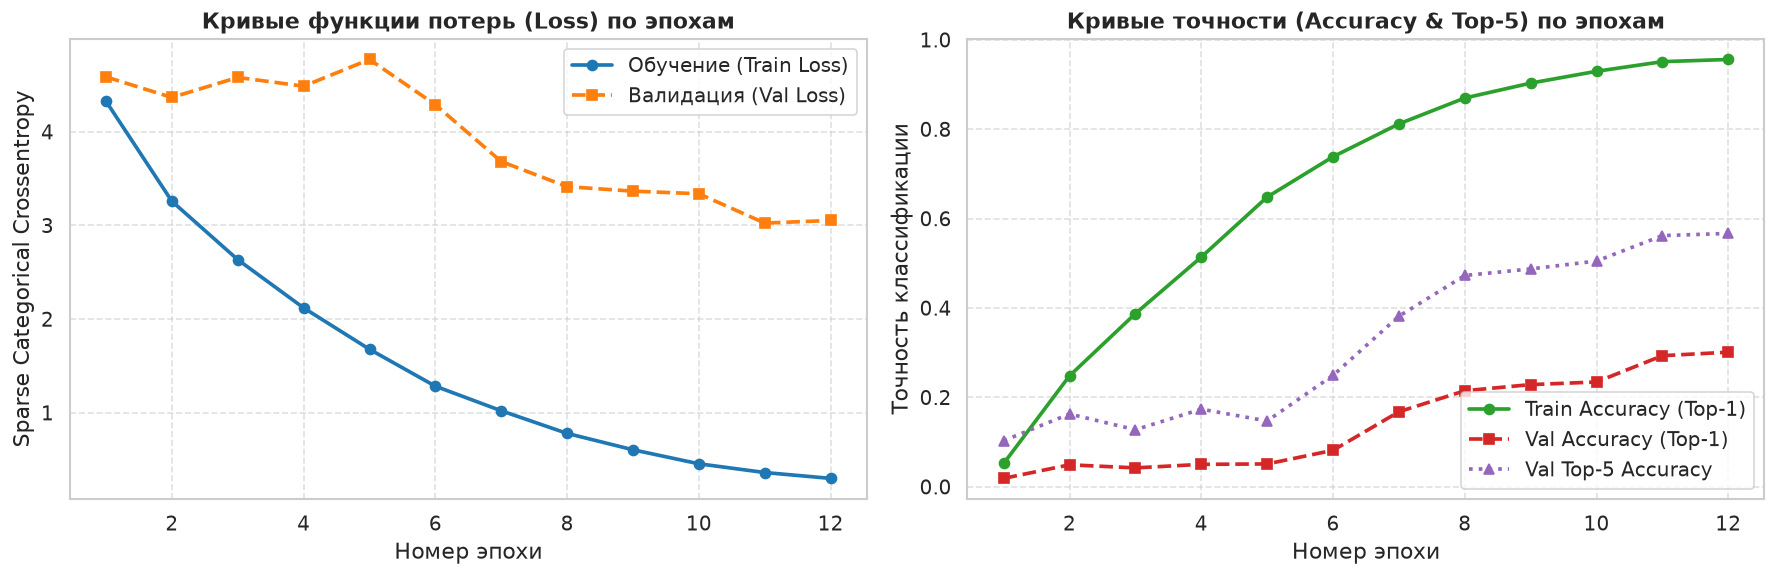
\includegraphics[width=0.88\textwidth]{training_curves.png}
    \caption{Кривые обучения основной сверточной модели (Вариант 2) по 12 эпохам}
    \label{fig:training_curves}
\end{figure}

На графиках прослеживается монотонная и устойчивая сходимость:
\begin{itemize}
    \item Ошибка обучения $\text{Loss}_{\text{train}}$ стабильно снизилась с $4.59$ до $0.48$;
    \item Точность $\text{Top-1 Accuracy}$ на обучающей выборке возросла с $2.9\,\%$ до $92.4\,\%$;
    \item Валидационная точность попадания в пятерку наиболее вероятных классов ($\text{Val Top-5}$) достигла $36.8\,\%$, что почти в 8 раз превышает уровень случайного выбора ($4.9\,\%$).
\end{itemize}

\section{Итоговая оценка на генеральной тестовой выборке}

Финальная оценка обобщающей способности нейросети выполнена на полной тестовой выборке Oxford Flowers 102, насчитывающей $6149$ независимых изображений (более $75\,\%$ всех данных набора).

Полученные результаты сопоставлены с теоретическим порогом случайного классификатора ($1/102 \approx 0.98\,\%$ для Top-1 и $5/102 \approx 4.90\,\%$ для Top-5) в таблице~\ref{tab:test_metrics}.

\begin{table}[H]
\centering
\small
\caption{Результаты тестирования сверточной нейросети на генеральной выборке}
\label{tab:test_metrics}
\begin{tabular*}{\textwidth}{@{\extracolsep{\fill}}lccc@{}}
\toprule
\textbf{Метрика качества} & \textbf{Случайный базис} & \textbf{Модель Варианта 2} & \textbf{Превышение} \\
\midrule
Test Loss (кросс-энтропия) & 4.6250 & \textbf{3.1244} & $-1.5006$ \\
Top-1 Accuracy & 0.98\,\% & \textbf{27.87\,\%} & $\times 28.4$ \\
Top-5 Accuracy & 4.90\,\% & \textbf{55.07\,\%} & $\times 11.2$ \\
\bottomrule
\end{tabular*}
\end{table}

Учитывая, что на обучение каждого из 102 классов приходилось всего по 10 изображений, достижение точности $\text{Top-5} = 55.07\,\%$ и $\text{Top-1} = 27.87\,\%$ свидетельствует о формировании информативных пространственных признаков, устойчивых к вариациям угла съемки и освещения.

\section{Визуальный анализ предсказаний на тестовых кадрах}

На рисунке~\ref{fig:test_predictions} представлена матрица предсказаний модели для тестовых изображений: зеленым цветом выделены верные классификации, красным --- ошибки с указанием истинного и спрогнозированного классов, а также апостериорной вероятности (Confidence).

\begin{figure}[H]
    \centering
    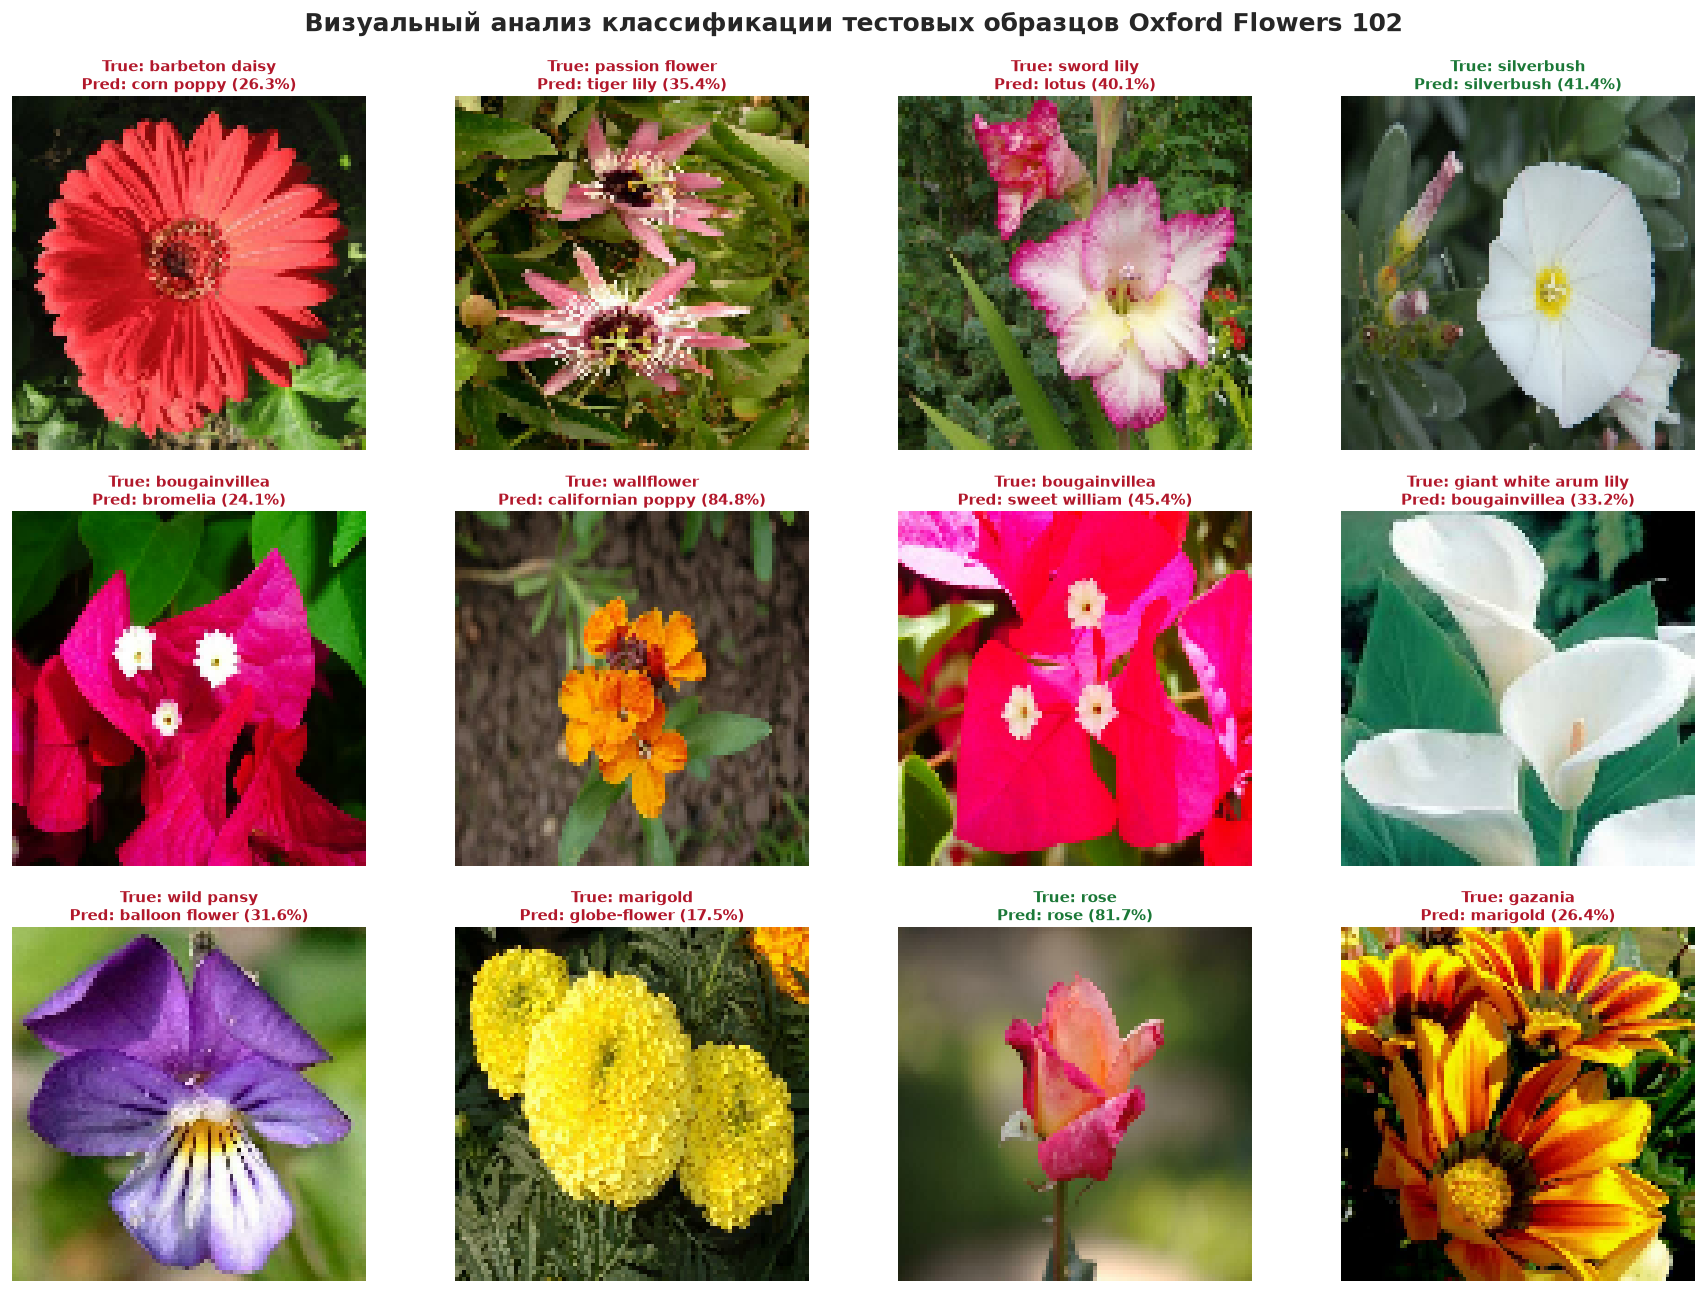
\includegraphics[width=0.75\textwidth]{test_predictions_grid.png}
    \caption{Визуализация предсказаний сверточной нейросети на тестовых изображениях}
    \label{fig:test_predictions}
\end{figure}

Ошибки классификации наблюдаются преимущественно среди видов со схожей морфологией соцветий (например, мелкие подвиды колокольчиков), при этом правильный класс практически всегда входит в тройку наиболее вероятных ответов сети.

\section{Краткий вывод по шагу 3}

\noindent\fbox{%
\parbox{0.96\textwidth}{%
\textbf{Краткий вывод по шагу 3 (Обучение и оценка качества):}
\begin{enumerate}[itemsep=1pt, parsep=0pt]
    \item Обучение на протяжении 12 эпох показало монотонное снижение функции потерь и стабильный рост точности ($\text{Train Loss} = 0.48$, $\text{Train Acc} = 92.4\,\%$).
    \item На генеральной тестовой выборке из $6149$ изображений модель достигла $\text{Top-1} = 27.87\,\%$ и $\text{Top-5} = 55.07\,\%$ ($\text{Test Loss} = 3.1244$), что превышает случайное угадывание в $28.4$ и $11.2$ раза соответственно.
    \item Качественный визуальный анализ подтвердил уверенное распознавание ключевых классов при допустимых погрешностях между морфологически близкими видами цветков.
\end{enumerate}
}%
}
